\documentclass{beamer}
\usepackage[british]{babel}
\usepackage{times}
\usepackage{amsmath}
\usepackage{mathtools}
\usepackage{amsfonts}
\usepackage{verbatim}
\usepackage{lmodern}
\usepackage{tikz}
%\usepackage{algorithm}
\usetikzlibrary{patterns}


\DeclareMathOperator*{\argmax}{arg\,max}
\DeclareMathOperator*{\argmin}{arg\,min}

\DeclareMathOperator*{\KL}{{\rm KL}}

\begin{document}
\title{Mid-term presentation}
\author{William van Rooij}
\institute{EPFL}
\date{12.04.19}
\logo{
\includegraphics[width=30px]{images/EPFL_Logo.png}}
\maketitle
\begin{frame}
\begin{itemize}
\item Introduction
\item Variational inference
\item Mean-field approximation
\item LOCUS R
\item Results
\item Future
\end{itemize}
\end{frame}
\begin{frame}
\frametitle{Introduction}
\begin{itemize}
\item Estimate the association between SNP $s$ and trait $t$,

$s = 1,\ldots,p$, $t=1,\ldots ,q$
\item $y_{n\times q} = x_{n\times p}\beta_{p \times q} + \epsilon_{n\times q}\text{, }\epsilon \sim \mathcal{N}(0,\tau_t^{-1}I_n)$
\item $y$ is response matrix, $x$ are candidate predictors.

\item Each response $y_t$ is linearly related with the predictors and has a residual precision $\tau_t \sim $ Gamma$(\eta_t, \kappa_t)$.

\item $p$ and $q$ really large compared $n$.
\end{itemize}
\end{frame}
\begin{frame}
\frametitle{Introduction II}
\begin{itemize}

\item $\beta_{st}\mid\gamma_{st},\sigma^2,\tau_t \sim \gamma_{st}\mathcal{N}(0,\sigma^2\tau_t^{-1})+(1-\gamma_{st})\delta_0$,

(spike and slab)

\item $\gamma_{st} \mid \omega_{s} \sim $ Bernoulli$(\omega_s)$,

\item $\omega_s \sim $ Beta$(a_s,b_s)$,

\end{itemize}

\end{frame}
\begin{frame}
\frametitle{Variational inference}
\begin{itemize}
\item Observed data $\boldsymbol{y}$, parameters $\boldsymbol{\theta}$, posterior distribution of parameters $p(\boldsymbol{\theta} \mid \boldsymbol{y})$.
\item Approximate posterior density with a simpler density $q$, minimizing a "closeness" measure: the Kullback-Leibler divergence.
\item $\KL(q\parallel p) := \int q(\boldsymbol{\theta})\log \left(\dfrac{q(\boldsymbol{\theta})}{p(\boldsymbol{\theta} \mid \boldsymbol{y})}\right) \mathrm{d}\boldsymbol{\theta}$.
\item Evidence lower bound (ELBO): $\mathcal{L}(q) = \mathbb{E}\left[\log p(\boldsymbol{\theta},\boldsymbol{y})\right] - \mathbb{E}\left[\log q(\boldsymbol{\theta})\right]$.
\item $\KL(q\parallel p) = \log(p) - \mathcal{L}(q)$.
\item Minimizing KL is equivalent to maximizing ELBO.
\end{itemize}
\end{frame}

\begin{frame}
\frametitle{Mean-field approximation}
\begin{itemize}
\item We assume $q(\boldsymbol{\theta}) = \prod_{j=1}^Jq_j(\theta_j)$, where $\left\lbrace\theta_j\right\rbrace$, $j=1,\ldots,J$ is a decomposition of $\boldsymbol{\theta}$.
\item The mean-field approximation does not compute the correlations between parameters.
\end{itemize}
\begin{figure}
\centering
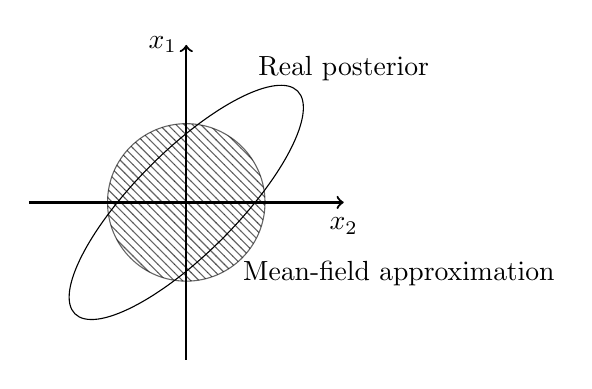
\begin{tikzpicture}
\draw[thick, ->] (0,-2) -- (0,2);
\draw[thick, ->] (-2,0) -- (2,0);
\fill[pattern=north west lines,opacity=.6,draw] (0,0) circle (1cm);
\draw[rotate=-45] (0,0) ellipse (0.65cm and 2cm);
\node (p) at (2,1.7) {Real posterior};
\node (q) at (2.7,-0.9) {Mean-field approximation};
\node (x1) at (-0.3,2) {$x_1$};
\node (x2) at (2,-0.3) {$x_2$};
\end{tikzpicture}\end{figure}
\end{frame}

\begin{frame}
\frametitle{Coordinate ascent variational inference - CAVI}
\begin{itemize}
\item If we fix $q_l(\theta_l)$, $l \neq j$, the optimal for $q_j(\theta_j)$ verifies: $q^*_j(\theta_j) \propto \exp\left\lbrace\mathbb{E}_{-j}\left[\log p(\theta_j \mid \boldsymbol{\theta}_{-j},\boldsymbol{y}\right]\right\rbrace$
\item \begin{text}
IN: $p(x,z)$, data set $x$, tolerance $tol$,\\
OUT: $q(z) = \prod q_j(z_j)$.\\
INIT: $q_j(z_j)$, \\
REPEAT:\\
\quad FOR: $j \in \left\lbrace1, \dots, m\right\rbrace$,\\
\quad \quad SET: $q_j(z_j) \propto \exp\left\lbrace\mathbb{E}_{-j}\left[\log p(z_j|z_{-j},x)\right]\right\rbrace$.\\
\quad COMPUTE:\\
\quad \quad $ELBO^{old}(q) \leftarrow ELBO(q)$.\\
\quad \quad $ELBO(q) = \mathbb{E}\left[\log p(z,x)\right] - \mathbb{E}\left[\log q(z) \right] $.\\
UNTIL: $|ELBO(q)-ELBO^{old}(q)|<tol$.\\
RETURN: $q(z).$
\end{text}
\end{itemize}
\end{frame}

\begin{frame}
\frametitle{Coordinate ascent variational inference - CAVI II}
\begin{itemize}
\item $\mathcal{L}(q)$ is guaranteed to augment at every iteration.
\item CAVI yields a local optimum, depending on the initialization of the parameters.
\begin{figure}
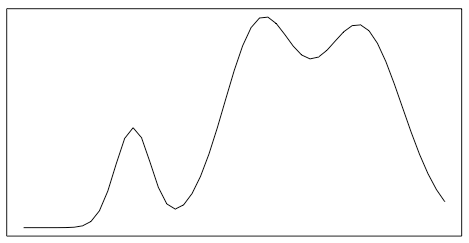
\includegraphics[width=3in]{images/localOptimum.png}
\end{figure}
\end{itemize}
\end{frame}

\begin{frame}
\frametitle{Bayesian model averaging}

\end{frame}



















\begin{frame}
\frametitle{ROC curves comparison, $p_0 = 15$, max var.$=0.5$}
\begin{figure}
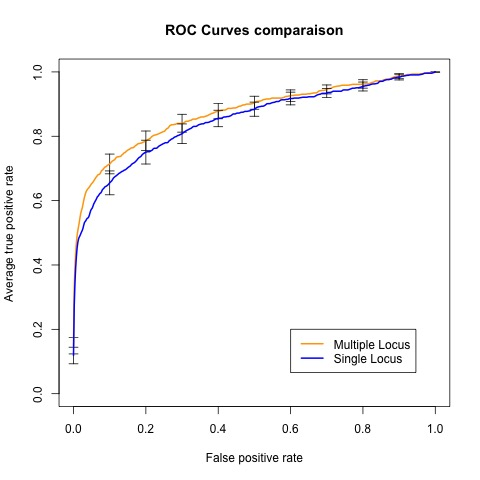
\includegraphics[width=3in]{images/ROC_Comp_p0_15_var_0_5.jpeg}
\end{figure}
\end{frame}
\begin{frame}
\frametitle{ROC curves comparison, $p_0 = 15$, max var.$=0.8$}
\begin{figure}
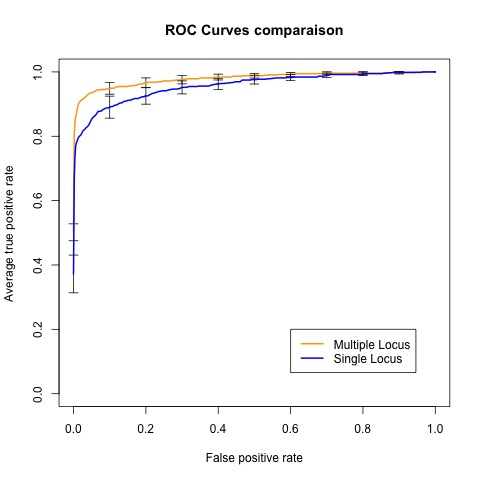
\includegraphics[width=3in]{images/ROC_Comp_p0_15_var_0_8.jpeg}
\end{figure}
\end{frame}
\begin{frame}
\frametitle{ROC curves comparison, $p_0 = 50$, max var.$=0.5$}
\begin{figure}
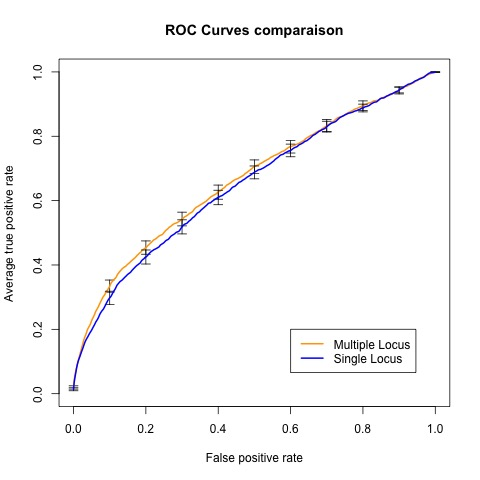
\includegraphics[width=3in]{images/ROC_Comp_p0_50_var_0_5.jpeg}
\end{figure}
\end{frame}
\begin{frame}
\frametitle{ROC curves comparison, $p_0 = 50$, max var.$=0.8$}
\begin{figure}
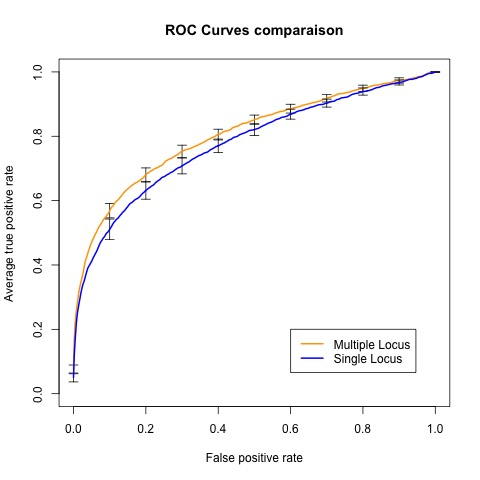
\includegraphics[width=3in]{images/ROC_Comp_p0_50_var_0_8.jpeg}
\end{figure}
\end{frame}
\end{document}